\documentclass[11pt, letterpaper]{article}
\usepackage[margin=0.5in]{geometry}
\usepackage{graphicx}

\begin{document}

\title{Assignment 3: Genetic Drift}
\author{Ryan Layer}
\maketitle

\section{Introduction}
Genetic drift is a mechanism of evolution that influences allele frequencies in
populations. It occurs due to random sampling of alleles during the formation
of gametes, leading to changes in allele frequencies in the subsequent
generation. Here we explore the effects of genetic drift on allele frequencies
using a simulation of random mating in a population. We observe that fixation
and loss of alleles occurs quickly even in the absence of selection.

\section{Results}
In a random mating simulation(Figure~ref{fig:drift} with no selection, five
samples, five loci where, and the number of offspring was center on two with a
standard deviation of one, two alleles were lost, and three reached fixation.

\begin{figure}[h]
    \centering
    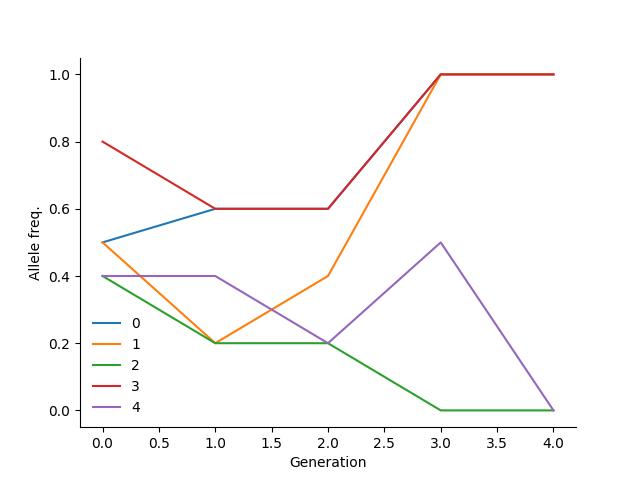
\includegraphics[width=0.5\textwidth]{fig1}
    \caption{The allele frequency of each generation of A random mating
    simulation with five samples, five loci, mean number of offspring of two,
    and standard deviation of one.}
    \label{fig:drift}
\end{figure}

\section{Methods}

Samples were represented by lists of alleles, where each was either a one or
zero, corresponding to the sample having or not having that allele. At each
generation, samples were randomly paired and the number of their offspring was
randomly selected from a normal distribution centered on mean number of
offspring with is specified by the user. For each offspring, alleles were
determined by randomly selecting a parental value. Once all offspring alleles
were set, the parents were removed from the simulation. At each round, the
allele frequency of each allele was determined by inspecting all of the
offspring.

Figure~\ref{fig:drift} visualizes the allele frequency at each generation for
one simulation with five samples, ten loci, mean number of offspring of two,
and standard deviation of one

To run the software, first clone the repository, then run the allele frequency
simulation as follows:
\begin{verbatim}
$ clone https://github.com/ryanlayerlab/drift.git
$ cd drift/src
$ python af.py \
  --num_samples 10 \
  --num_sites 5 \
  --mean_offspring 2 \
  --stdev_offspring 1 \
  --out_file af.png
\end{verbatim}

\end{document}
